%---------------------
\pagestyle{plain}
\setcounter{page}{1}
\pagenumbering{arabic}
%---------------------

\chapter{مقدمه و مفاهیم اولیه}

در این فصل به عنوان مقدمه، روش وارسی مدل به‌طور مختصر معرفی شده‌است. در فصل‌های بعدی، با هدف بهبود این روش، صورت‌های جدیدی از آن ارائه شده و مورد بررسی قرار گرفته است، بنابراین، لازم است که ابتدا، به معرفی این روش به شکل سنتی پرداخته شود.

پس از معرفی وارسی مدل، بحث اصلی این پایان نامه شروع می‌شود. محوریت کار ما\cite{calcul} است که در آن روش جدید وارسی مدل ارائه شده است. بحث با ارائه‌ی یک زبان شروع می‌شود، سپس معناشناسی رد پیشوندی برای این زبان ارائه می‌شود و فصل تمام می‌شود. مفاهیم معرفی شده در این فصل دارای ریزه‌کاری‌های زیادی هستند و به عقیده‌ی نگارنده، در \cite{calcul} در ارائه‌ی بعضی از جزئیات سهل انگاری اتفاق افتاده است. سعی کرده‌ایم که اگر ایرادی در تعاریف موجود در \cite{calcul} هست، حین بیان دوباره‌ی آن مفاهیم در این پایان نامه رفع کنیم، تا یک بیان خوش ساخت و روان از این نظریه ارائه کرده باشیم.


\section{روش وارسی مدل}

روش وارسی مدل یک روش صوری است که برای درستی‌یابی سیستم‌های مختلف استفاده می‌شود. در این روش معمولا ابتدا یک ماشین حالات متناهی از روی سیستم مورد بررسی ساخته می‌شود، سپس بررسی‌هایی که قرار است روی سیستم اصلی انجام شوند، روی این ماشین( مدل) انجام می‌شود. 

از این روش در بررسی صحت کارکرد برنامه‌های کامپیوتری استفاده می‌شود، اما این تنها مورد استفاده‌ی این روش نیست. و هر سیستمی که قابلیت بیان شدن به صورت صوری را داشته باشد، با این روش قابل بررسی است. مثلا می‌توان از این روش برای بررسی صحت عملکرد یک برنامه برای قطارهای شهری استفاده کرد. در یک برنامه‌ برای قطارهای شهری، نباید امکان حضور دو قطار روی یک ریل در یک زمان وجود داشته باشد( که معنی تصادف بین دو قطار را می‌دهد) و می‌توان از روش وارسی مدل برای اطمینان از عدم وجود چنین ویژگی نامطلوبی استفاده کرد. مثال های دیگر استفاده‌ی این روش در علوم کامپیوتر بررسی صحت عملکرد یک پردازنده یا الگوریتم تقسیمِ وظایف یک سیستم عامل است. این مثال‌ها هیچ کدام یک برنامه‌ی کامپیوتری نیستند( هر چند که ممکن است مجبور باشیم از یک برنامه‌ی کامپیوتری برای پیاده سازی آن‌ها کمک بگیریم که در آن صورت بررسی صحت عملکرد آن برنامه‌ی کامپیوتری داستانی دیگر خواهد داشت)، اما قابل بیان به صورت صوری به جای زبان طبیعی هستند.

روش وارسی مدل برای بیان خواص مورد بررسی از منطق‌های زمانی مختلف استفاده می‌کند. منطق زمانی یک نوع منطق موجهات است. منطق‌های موجهات از گسترش زبان منطق کلاسیک، با اضافه کردن ادات وجهی گوناگون، ساخته می‌شوند. این ادوات غالبا در زبان طبیعی نقش قید را دارند. منطق‌های زمانی دسته‌ای از منطق‌های موجهات هستند که به صوری‌گری ما مفهوم زمان را اضافه می‌کنند، یعنی قیدهایی مانند فعلا، بعدا، و قبلا( که مورد آخری کمتر رایج است). منطقی که در اینجا بیان می‌کنیم \lr{LTL} نام دارد که یکی از منطق‌های زمانی است که برای روش وارسی مدل استفاده می‌شود. البته در مورد قیدهای مذکور، اشاره به این نکته ضروری است که در بیانی که در اینجا از این منطق ارائه داده‌ایم، ادوات جدید به‌طور مستقیم بیانگر این قید‌ها نیستند، هرچند که به کمک ادوات جدید می‌توان ادواتی برای هر یک از این قیود ساخت.
این تعاریف از \cite{buchi} آورده شده‌اند.

ابتدا زبان این منطق را بیان می‌کنیم و سعی می‌کنیم، به طور غیر دقیق، در مورد معنای فرمول‌های این زبان به خواننده یک درک شهودی بدهیم، سپس به سراغ معناشناسی صوری این منطق می‌رویم.

\subsection{زبان \lr{LTL}}
\begin{defn}
	هر عضو مجموعه‌ی $\Phi$ یک فرمول در زبان \lr{LTL} است( و $\Pi$ مجموعه‌ی‌( شمارای نامتناهی) فرمول‌های اتمی است و $\pi \in \Pi$):
	$$
	\Pi \subset \Phi,
	$$
	$$
	\phi \in \Phi \Leftrightarrow
	\phi ::= \pi | \phi \lor \phi |
	\neg \phi |
	\bigcirc \phi |
	\phi \mathcal{U}\phi 
$$	
	
\end{defn}
در این منطق، ما زمان را با اعداد طبیعی نشان می‌دهیم. یعنی برای یک فرمول، زمان از عدد ۰ شروع شده و تا ابد ادامه خواهد داشت و حین گذر زمان ممکن است ارزش فرمول‌ها تغییر کند. مسلما پس از بررسی معناشناسی صوری بهتر می‌شود این مفهوم را به طور شهودی حس کرد، اما به هر حال به خواننده پیشنهاد می‌شود، پیش از رسیدن به آن بخش به ادامه‌ی این بخش که در تلاش است یک درک شهودی از معنای فرمول‌ها بدهد، توجه کند. 

در این زبان ادوات کلاسیک 
$\neg, \lor$
هستند با همان معنایی که در منطق گزاره‌ای کلاسیک داشتند.  
در ادوات جدید 
$\bigcirc \phi$
به معنای برقرار بودن این فرمول دقیقا در لحظه‌ی بعدی( دقیقا یک لحظه) است، مثلا در شکل زیر با در نظر گرفتن اینکه در زمان 0 هستیم، این فرمول در لحظه‌ی ۱ برقرار است.
	\begin{center}
	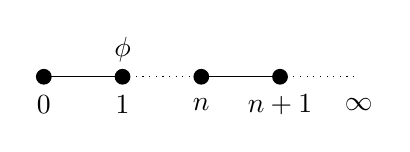
\begin{tikzpicture}
	\node at (1,0.35) (phi) {$\phi$};
	\node at (1,-0.35) (1) {$1$};
	\node at (0,-0.35) (0) {$0$};
	\node at (2,-0.35) (n) {$n$};
	\node at (3,-0.35) (1) {$n+1$};
	\node at (4,-0.35) (1) {$\infty$};
	\fill (0,0) circle (0.1cm);
	\fill (1,0) circle (0.1cm);
	\fill (2,0) circle (0.1cm);
	\fill (3,0) circle (0.1cm);
	\path (0,0) edge (1,0) 
	(1,0) edge[dotted] (2,0)
	(2,0) edge (3,0)
	(3,0) edge[dotted] (4,0);
	\end{tikzpicture}
\end{center}
$\phi \mathcal{U}\psi$
به این معنی است که فرمول سمت چپی حداقل تا قبل از اینکه فرمول سمت راستی برقرار شود، برقرار است.( مثلا اگر بگوییم "تا وقتی که باران نباریده زمین خشک است" در این صورت "زمین خشک است" به جای فرمول سمت چپ و "باران باریده است" فرمول سمت راست است).
\begin{center}
	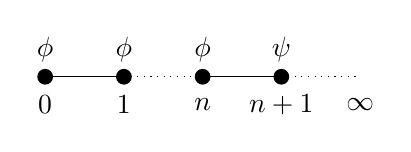
\begin{tikzpicture}
	\node at (1,0.35) (phi) {$\phi$};
	\node at (0,0.35) (phi) {$\phi$};
	\node at (2,0.35) (phi) {$\phi$};
	\node at (3,0.35) (phi) {$\psi$};
	\node at (1,-0.35) (1) {$1$};
	\node at (0,-0.35) (0) {$0$};
	\node at (2,-0.35) (n) {$n$};
	\node at (3,-0.35) (1) {$n+1$};
	\node at (4,-0.35) (1) {$\infty$};
	\fill (0,0) circle (0.1cm);
	\fill (1,0) circle (0.1cm);
	\fill (2,0) circle (0.1cm);
	\fill (3,0) circle (0.1cm);
	\path (0,0) edge (1,0) 
	(1,0) edge[dotted] (2,0)
	(2,0) edge (3,0)
	(3,0) edge[dotted] (4,0);
	\end{tikzpicture}
\end{center}

این زبان را می‌توان با ادوات بیشتری از آنچه آورده‌ایم بیان کرد و البته بیان‌های دیگری هم بسته به بحث متداول هستند، اما در اینجا یک شکل ساده از این زبان را آورده‌ایم که به غیر از ادوات منطق گزاره‌ای دو ادات دیگر را در زبان خود دارد. دلیل وجود ادوات متفاوت، می‌تواند راحت‌تر کردن بیان خواص باشد. همان طور که استفاده نکردن از یا و شرطی در منطق گزاره‌ای می‌تواند به سخت کردن بیان جملات در چارچوب این منطق منجر شود، حذف این ادوات وجهی هم بیان خواص را در این منطق مشکل می‌سازد. 

حال که به درکی شهودی از معنای فرمول‌های این زبان رسیده‌ایم، به بیان صوری این مفاهیم می‌پردازیم.

\subsection{معناشناسی \lr{LTL}}

مدل‌های این منطق را به صورت توابع
$M:\mathbb{N}_0 \rightarrow \mathit{P}(\Pi)$ 
تعریف می‌کنیم. به عبارت دیگر، هر مدل یک تابع است که هر عدد طبیعی را به یک مجموعه از فرمول‌های اتمی می‌برد. این در واقع به این معنی است که یک مدل مشخص می‌کند که در هر لحظه کدام یک از فرمول‌های اتمی درست هستند. مثلا، در مدلی به نام $M$ در واقع
$M(5)$
مجموعه‌ی اتم‌هایی است که در لحظه‌ی 5 طبق این مدل درست هستند و اگر اتمی در این مجموعه حاضر نباشد، در لحظه‌ی 5، ارزش غلط دارد.
درستی یک فرمول در یک مدل را با 
$M,i$
نشان می‌دهیم و 
$M,i \models \phi$
به این معنی است که فرمول $\phi$، در لحظه‌ی $i$در مدل $M$ ارزش درست دارد. این مفهوم را، به صورت بازگشتی، به شکل زیر تعریف می‌کنیم:


\begin{flushleft}
$	M,i \models \pi \:\:\: \mathit{iff} \:\:\: \pi \in M(i)$\\
$	M,i \models \neg \phi \:\:\: \mathit{iff} \:\:\: M,i\nvDash \phi$\\
$	M,i \models \phi \lor \psi \:\:\: \mathit{iff} \:\:\: M,i \models \phi \:\:\: \mathit{or} \:\:\: M,i \models \psi$\\
	 $M,i \models \bigcirc \phi  \:\:\:  \mathit{iff} \:\:\: M,i+1 \models \phi$\\
	 $M,i \models \phi \mathcal{U} \psi \:\:\: \mathit{iff} \:\:\: 
	 \exists k \geq i \in \mathbb{N}_0: \forall i\leq j< k: M,j \models \phi \:\:\: \mathit{and} \:\:\: M,k \models \psi$
\end{flushleft}


یک فرمول را ارضاپذیر می‌گوییم اگر و تنها اگر مدلی وجود داشته باشد که فرمول در آن صادق باشد.
اگر یک فرمول در هر مدلی صادق باشد، آن فرمول را \emph{معتبر} می‌گوییم.\\



\section{نحو زبان مورد بررسی‬}
زبان بیان برنامه ها زیرمجموعه ای از دستورات زبان \lr{C} است، به شکل زیر:
$$\mathsf{x,y},... \in \mathbb{X}\hspace{4.65cm}$$
$$\mathsf{A} \in \mathbb{A} ::=\mathsf{1\:|\:x\:|\:A_1 - A_2\hspace{2.4cm}}$$  
$$\mathsf{B \in \mathbb{B} ::=A_1<A_2 \:|\: B_1 \: nand\: B_2\hspace{1.2cm}}$$
$$\mathsf{E \in \mathbb{E}::= A \: | \: B\hspace{4cm}}$$
$$\mathsf{S\in \mathbb{S} ::=\hspace{5cm}  }$$
$$\mathsf{x\doteq A; \hspace{2.25cm}}$$
$$\mathsf{|\:\:\:;\hspace{3.75cm}}$$
$$\mathsf{|\:\:\:if\:(B)\:S\:|\:if\:(B)\:S\:else\:S}$$
$$\mathsf{|\:\:\:while\:(B)\:S\: | \: break;\hspace{0.65cm}}$$
$$\mathsf{|\:\:\:\{Sl\}\hspace{3.15cm}}$$
$$\mathsf{Sl \in \mathbb{SL}::=Sl\:\:\:S\:|\:\backepsilon}\hspace{3.05cm}$$
$$\mathsf{P\in \mathbb{P}\:::=Sl}\hspace{4.25cm}$$

\vspace{1cm}
قابل مشاهده است که این زبان، نسبت به کل زبان \lr{C}، تا حد ممکن ساده سازی شده است. علت این کار را بعدا عمیق‌تر حس خواهیم‌کرد. علتْ ساده‌تر شدن کار برای ارائه‌ی معناشناسی و صورت‌های جدید روش وارسی مدل است. در اینجا، راحتی برنامه نوشتن در این زبان مطرح نبوده است، چون اصلا این زبان برای این کار ساخته نشده است. هدف ارائه‌ی این زبان صرفا ارائه‌ی روش جدید است. یعنی می‌توان به این زبان به چشم یک مدل محاسباتی، مانند ماشین تورینگ و ماشین رجیستر، نگاه کرد. روشی که سعی در ارائه‌اش داریم، برای زبان‌های برنامه نویسی دستوری است، مانند پایتون، جاوا و \lr{C}. بنابراین، انتخاب یک مدل محاسباتی که به رفتاری شبیه‌تر به این زبان‌ها داشته باشد، کار معقولی است.

اندکی در مورد قدرت بیان این زبان صحبت می‌کنیم. می‌توانیم باقی اعداد را از روی عدد ۱ و عملگر منها بسازیم. مثلا ابتدا 0 را به کمک ۱-۱ می سازیم و سپس با استفاده از 0 می‌توانیم یکی یکی اعداد منفی را بسازیم و سپس بعد از آن به سراغ اعداد مثبت می‌رویم که با کمک 0 و هر عدد منفی‌ای که ساختیم، ساخته می شوند. باقی اعداد و حتی باقی عملگر‌ها( یعنی به غیر از اعداد طبیعی) نیز از روی آنچه داریم قابل‌ساختن است. در مورد عبارت‌های بولی نیز داستان به همین منوال است. یعنی اینجا صرفا ادات شفر تعریف شده و باقی عملگر‌های بولی را می‌توان با استفاده از همین عملگر ساخت. باقی دستورات نیز دستورات شرط و حلقه هستند. باقی دستورات مطابق رفتاری که از آن‌ها در زبان \lr{C} انتظار داریم کار می‌کنند. در مورد دستور \lr{$\mathsf{break;}$} ذکر این نکته ضروری است که اجرای آن اجرای برنامه را از دستوری بعد از داخلی‌ترین حلقه‌ای که \lr{$\mathsf{break;}$} داخلش قرار دارد ادامه می‌‌دهد. در پایان می توان ثابت کرد که این زبان هم قدرت با ماشین تورینگ\cite{davis} است. 

توجه داریم که هر‌چه در بالا در‌مورد معنای دستورات این زبان گفتیم، به هیچ وجه صوری نیست. صرفا درک شهودی‌ای که از معنای اجرای هر‌یک از دستورات می‌توان داشت را بیان کرده‌ایم. بیان صوری معنای برنامه‌ها را که خلاف درک شهودی‌مان قابل انتقال به کامپیوتر‌ است، در ادامه بیان خواهیم‌کرد. طبیعتا، این بیان صوری از روی یک درک شهودی ساخته شده‌است.

\section{معناشناسی زبان مورد بررسی‬}
معناشناسی زبانی را که در بخش پیش آورده‌ایم، با کمک مفاهیمی به نام‌های "برچسب" و "رد پیشوندی" و عملگری به نام "چسباندن" تعریف می‌کنیم. نام این معناشناسی "معناشناسی رد پیشوندی" است.\\

\subsection{برچسب‌ها}

با‌وجود اینکه در زبان \lr{C} مفهوم برچسب، که می‌خواهیم معرفی اش کنیم، وجود دارد،اما در زبانی که معرفی کردیم، خبری از برچسب‌ها نبود. با این وجود، برای تعریف صوری معنای برنامه‌ها، به این مفهوم نیاز داریم. در این بخش، به‌طور غیر دقیق معنای برچسب‌ها را آورده‌ایم. همین تعاریف غیر دقیق برای کار ما کافی است. تعاریف صوری دقیق‌تر این موجودات در پیوست \cite{calcul} آورده‌شده‌اند. از آوردن مستقیم این تعاریف در اینجا خود‌داری کرده‌ایم. البته در مورد معنای صوری برجسب‌ها قابل ذکر است که طبق \cite{cousotbook}، تعریف صوری برچسب‌ها غیر قطعی است. به عبارت دیگر، این تعریف ناکامل است و سیستم‌های صوری متفاوتی را می‌توان متصور شد که در تعریف صوری برچسب‌ها می‌گنجند.

در زبانمان، \lr{$\mathsf{S}$}ها بخشی از عبارات موجود در زبان هستند. برچسب ها را برای \lr{$\mathsf{S}$}ها تعریف می‌کنیم. برچسب‌ها با کمک توابع \lr{labs, in, brks-of, brk-to, esc, aft, at} تعریف می‌شوند. در‌ واقع، هر $\mathsf{S}$، به ازای هر یک از این توابع، ممکن است یک برجسب متفاوت داشته باشد. بعضی دیگر از این توابع به ازای هر $\mathsf{S}$ ممکن است یک مجموعه از برچسب‌ها را برگردانند. یکی از آن‌ها هم با گرفتن $\mathsf{S}$ یک مقدار بولی را بر‌می‌گرداند. 
\\\\
\lr{at$\llbracket\mathsf{S}\rrbracket$} : برچسب شروع $\mathsf{S}$.\\
\lr{aft$\llbracket\mathsf{S}\rrbracket$} : برچسب پایان $\mathsf{S}$، اگر پایانی داشته باشد.\\
\lr{esc$\llbracket\mathsf{S}\rrbracket$} : یک مقدار بولی را باز‌‌می‌گرداند که بسته به اینکه در $\mathsf{S}$ دستور $\mathsf{break;}$ وجود دارد یا خیر، مقدار درست یا غلط را بر‌می‌گرداند.\\
\lr{brk-to$\llbracket\mathsf{S}\rrbracket$} : 
برچسبی است که اگر حین اجرای $\mathsf{S}$ دستور $\mathsf{break;}$ اجرا شود، برنامه از آن نقطه ادامه پیدا می کند.\\
\lr{brks-of$\llbracket\mathsf{S}\rrbracket$} :
مجموعه‌ای از برچسب دستورات
$\mathsf{break;}$
های داخل $\mathsf{S}$ را بر‌می‌گرداند.\\
\lr{in$\llbracket\mathsf{S}\rrbracket$} : مجموعه‌ای از تمام برچسب‌های درون $\mathsf{S}$ را برمی‌گرداند.\\
\lr{labs$\llbracket\mathsf{S}\rrbracket$} : مجموعه‌ای از تمام بر‌چسب‌هایی که با اجرای $\mathsf{S}$ قابل دسترسی هستند را بر‌می‌گرداند.\\\\\\
مجموعه‌ی همه‌ی برچسب‌ها را با 
$\mathbb{L}$
نشان می‌دهیم.

\subsection{رد پیشوندی}


حال که تعریف برچسب‌ها را هم داریم، به سراغ تعریف رد پیشوندی می‌رویم. البته پیش از آن، باید وضعیت‌ها و محیط‌ها را تعریف کنیم.
\begin{defn}
	(محیط): به ازای مجموعه مقادیر $\mathbb{V}$ و مجموعه متغیرهای $\mathbb{X}$ تابع 
	$\rho : \mathbb{X} \rightarrow \mathbb{V}$ 
	را یک محیط می‌گوییم. مجموعه‌ی همه‌ی محیط‌ها را با $\mathbb{EV}$ نمایش می‌دهیم.
\end{defn}

\begin{defn}
	(وضعیت): به هر زوج مرتبْ به ترتیب متشکل از یک برچسب $l$ و یک محیط $\rho$ یک وضعیت (یا حالت)  
	$\langle l , \rho \rangle$
	می‌گوییم. مجموعه‌ی همه‌ی وضعیت‌ها را با $\mathfrak{S}$ نشان می‌دهیم.
\end{defn}
\begin{defn}
	(رد پیشوندی): به یک دنباله از وضعیت‌ها(با امکان تهی بودن) یک رد پیشوندی می‌گوییم.
\end{defn}

هر رد پیشوندی یک دنباله است که قرار است توصیفی از چگونگی اجرای برنامه باشد. وضعیت‌ها موقعیت لحظه‌ای حافظه‌ا‌ی در دسترس برنامه است را توصیف می‌کنند. $l$ برچسب قسمتی از برنامه‌ است که در حال اجرا است و $\rho$ مقدار متغیر‌ها را در آن موقع از اجرای برنامه نشان می‌دهد. دنباله‌های ما می‌توانند متناهی یا نامتناهی باشند. مجموعه‌ی ردهای پیشوندی‌ متناهی را با $\mathfrak{S^+}$ و مجموعه‌ی ردهای پیشوندی نامتناهی را با  $\mathfrak{S^\infty}$ نمایش می‌دهیم. مجموعه‌ی همه‌ی ردهای پیشوندی را هم با $\mathfrak{S^{+\infty}}$ نمایش می‌دهیم. 
با‌توجه به آنچه گفتیم، یک عملگر چسباندن $\Join$ را روی ردهای پیشوندی تعریف می‌کنیم. 

پیش از ارائه‌ی تعریف، به دو نکته‌ی مهم در مورد نمادگذاری‌های این پایان نامه اشاره می‌کنیم.

اولین نکته این است که حین ارائه‌ی تعریف‌ها، مانند تعریف عملگر چسباندن که در ادامه آمده، اگر تعریف را روی یک ساختار یا با در نظر گرفتن پیش فرض‌های مختلف ارائه داده باشیم، ابتدا، هر فرض را با علامت 
$\blacktriangleleft$
نشان داده‌ایم. در اثبات‌ها به جای این نماد از 
$\blacktriangleright$
استفاده کرده‌ایم. 

نکته‌ی دوم در مورد نشان دادن ردهای پیشوندی است. اگر $\pi_1,\pi_2$ رد پیشوندی باشند و $\sigma$ یک وضعیت باشد، $\pi_1\sigma$ به یک رد پیشوندی لزوما متناهی اشاره می‌کند که با وضعیت $\sigma$ به پایان رسیده است،
$\sigma\pi_1$
به یک رد پیشوندی اشاره می‌کند که با وضعیت $\sigma$ شروع شده است و $\pi_1\pi_2$ به یک رد پیشوندی اشاره می‌کند که با $\pi_1$ شروع شده است و با $\pi_2$ ادامه پیدا می‌کند( $\pi_1$ باید متناهی باشد). توجه شود که $\pi_1\pi_2$ با چسباندن $\pi_1$ و $\pi_2$ $(\pi_1 \Join \pi_2)$به همدیگر متفاوت است.

\begin{defn}
	(عملگر چسباندن): اگر داشته باشیم 
	$\pi_1 , \pi_2 \in \mathfrak{S^{+\infty}}  , \sigma_1 ,\sigma_2 \in \mathfrak{S}$
	داریم:\\
	\begin{center}
		
		$$\blacktriangleleft \pi_1 \in \mathfrak{S}^\infty:$$
		$$\pi_1 \Join \pi_2 = \pi_1$$
		$$\blacktriangleleft \pi_1 \in \mathfrak{S}^+:$$
		$$\blacktriangleleft \blacktriangleleft \sigma_1 = \sigma_2:$$
		$$\pi_1\sigma_1 \Join \sigma_2 \pi_2 = \pi_1 \sigma_1 \pi_2$$
		$$\blacktriangleleft \blacktriangleleft \sigma_1 \neq \sigma_2:$$
		در این حالت 
		$\pi_1 \Join \pi_2$
		تعریف نمی‌شود.
	\end{center}
\end{defn}
همینطور، $\epsilon$ یک رد پیشوندی است که حاوی هیچ وضعیتی نیست. به عبارت دیگر، یک دنباله‌ی تهی است.

\subsection{تعریف صوری معناشناسی رد پیشوندی}
در این بخش، دو تابع $\mathcal{A}$ و $\mathcal{B}$ را به ترتیب روی عبارات حسابی و بولی زبانمان ، یعنی $\mathsf{A}$ها و $\mathsf{B}$ها تعریف می‌کنیم، سپس با کمک آنها $\mathcal{S^*}$ را روی  مجموعه‌ای از اجتماع معنای $\mathsf{S}$ها و $\mathsf{Sl}$ها تعریف می کنیم. پس در نهایت، هدف ما تعریف  $\mathcal{S^*}$ است.


\begin{defn}
	(معنای عبارات حسابی - تابع $\mathcal{A}$): تابع 
	$\mathcal{A}:\mathbb{A}\rightarrow \mathbb{EV} \rightarrow \mathbb{V}$
	را به صورت بازگشتی روی ساختار 
	$\mathsf{A} \in \mathbb{A}$
	به شکل زیر تعریف می‌کنیم:
	$$\mathcal{A\llbracket\mathsf{1}\rrbracket\rho = }1     $$
	$$\mathcal{A\llbracket\mathsf{x}\rrbracket\rho = } \rho(\mathsf{x})          $$
	$$\mathcal{A\llbracket\mathsf{A_1-A_2}\rrbracket\rho = }\mathcal{A\llbracket\mathsf{A_1}\rrbracket\rho }- \mathcal{A\llbracket\mathsf{A_2}\rrbracket\rho }       $$
	
\end{defn}

\begin{defn}
	(معنای عبارات بولی - تابع $\mathcal{B}$): تابع 
	$\mathcal{B}: \mathbb{B} \rightarrow \mathbb{EV} \rightarrow \mathbb{BOOL}$
	را به صورت بازگشتی روی ساختار 
	$\mathsf{B} \in \mathbb{B}$
	به شکل زیر تعریف می‌کنیم:
	
	\begin{center}
		اگر $\mathcal{A\llbracket\mathsf{A_1}\rrbracket\rho }$ کوچکتر از $\mathcal{A\llbracket\mathsf{A_2}\rrbracket\rho }$ باشد
		$\mathcal{B\llbracket\mathsf{A_1<A_2}\rrbracket\rho = } True   \hspace{2cm}  $\\
		اگر $\mathcal{A\llbracket\mathsf{A_1}\rrbracket\rho }$ بزرگتر از $\mathcal{A\llbracket\mathsf{A_2}\rrbracket\rho }$ باشد
		$\mathcal{B\llbracket\mathsf{A_1<A_2}\rrbracket\rho = } False   \hspace{2cm}  $\\
		$ \mathcal{B\llbracket\mathsf{B_1 nand B_2}\rrbracket\rho = } \neg(\mathcal{B\llbracket\mathsf{B_1}\rrbracket\rho}   \wedge \mathcal{B\llbracket\mathsf{B_2}\rrbracket\rho}) $
	\end{center}
\end{defn}

طبیعتا $\wedge$ و $\neg$ در فرازبان هستند.\\

در ادامه، به تعریف $\mathcal{S^*}$ می‌پردازیم. این کار را با تعریف $\mathcal{S^*}$ روی هر ساخت $\mathsf{S}$ و $\mathsf{Sl}$ انجام می‌دهیم.
پیش از ادامه‌ی بحث، باید این نکته را در‌مورد علامت‌گذاری‌هایمان ذکر کنیم که منظور از $        \mathsf{S} ::= l \mathsf{break;}  $ این است که تاکید کرده‌ایم که $\mathsf{S}$ با برچسب $l$ شروع شده‌است، هرچند که همین طور که پیش‌تر گفته‌شد،   $l$ جزو زبان نیست.\\\\

\begin{defn}
	(معنای برنامه‌ها - تابع $\mathcal{S}^*$): 
	اگر $        \mathsf{S} ::= \mathsf{break;}  $ باشد، ردهای پیشوندی متناظر با اجرای این دستور را به شکل مجموعه‌ی زیر تعریف می‌کنیم:
	$$\mathcal{S^*} \llbracket\mathsf{S}\rrbracket = \{ \langle at\llbracket\mathsf{S}\rrbracket , \rho \rangle | \rho \in \mathbb{EV}       \} \cup     \{ \langle at\llbracket\mathsf{S}\rrbracket , \rho \rangle \langle brk-to\llbracket\mathsf{S}\rrbracket , \rho \rangle | \rho \in \mathbb{EV}       \}             $$   
	
	
	اگر $        \mathsf{S} ::=  \mathsf{x\doteq A;}  $ باشد، ردهای پیشوندی متناظر با اجرای این دستور را به شکل مجموعه‌ی زیر تعریف می‌کنیم:
	$$\mathcal{S^*} \llbracket\mathsf{S}\rrbracket = \{ \langle at\llbracket\mathsf{S}\rrbracket , \rho \rangle | \rho \in \mathbb{EV}       \} \cup     \{ \langle at\llbracket\mathsf{S}\rrbracket , \rho \rangle \langle aft\llbracket\mathsf{S}\rrbracket , \rho[\mathsf{x}\leftarrow \mathcal{A}\llbracket\mathsf{A}\rrbracket\rho] \rangle | \rho \in \mathbb{EV}       \}             $$   
	
	اگر $         \mathsf{S} ::= \mathsf{if}  \mathsf{ (B) S_t}  $ باشد، ردهای پیشوندی متناظر با اجرای این دستور را به شکل مجموعه‌ی زیر تعریف می کنیم:
	$$\mathcal{S^*} \llbracket\mathsf{S}\rrbracket = \{ \langle at\llbracket\mathsf{S}\rrbracket , \rho \rangle | \rho \in \mathbb{EV}       \} \cup     \{ \langle at\llbracket\mathsf{S}\rrbracket , \rho \rangle \langle aft\llbracket\mathsf{S}\rrbracket , \rho \rangle | \mathcal{B}\llbracket\mathsf{B}\rrbracket \rho =False      \} 
	$$$$\cup    \{ \langle at\llbracket\mathsf{S}\rrbracket , \rho \rangle \langle at\llbracket\mathsf{S_t}\rrbracket , \rho \rangle 
	\pi | \mathcal{B}\llbracket\mathsf{B}\rrbracket \rho =True  \wedge   \langle  at\llbracket\mathsf{S_t}\rrbracket  , \rho \rangle \pi \in \mathcal{S} \llbracket\mathsf{S_t}\rrbracket    \}          $$ 
	
	
	اگر $         \mathsf{S} ::= \mathsf{if}  \mathsf{ (B) S_t else S_f}  $ باشد، ردهای پیشوندی متناظر با اجرای این دستور را به شکل مجموعه‌ی زیر تعریف می کنیم:
	$$\mathcal{S} \llbracket\mathsf{S}\rrbracket = \{ \langle at\llbracket\mathsf{S}\rrbracket , \rho \rangle | \rho \in \mathbb{EV}       \} $$$$\cup     \{ \langle at\llbracket\mathsf{S}\rrbracket , \rho \rangle \langle at\llbracket\mathsf{S_f}\rrbracket , \rho \rangle 
	\pi | \mathcal{B}\llbracket\mathsf{B}\rrbracket \rho =False  \wedge   \langle  at\llbracket\mathsf{S_f}\rrbracket  , \rho \rangle \pi \in \mathcal{S} \llbracket\mathsf{S_f}\rrbracket    \}  
	$$$$\cup    \{ \langle at\llbracket\mathsf{S}\rrbracket , \rho \rangle \langle at\llbracket\mathsf{S_t}\rrbracket , \rho \rangle 
	\pi | \mathcal{B}\llbracket\mathsf{B}\rrbracket \rho =True  \wedge   \langle  at\llbracket\mathsf{S_t}\rrbracket  , \rho \rangle \pi \in \mathcal{S} \llbracket\mathsf{S_t}\rrbracket    \}          $$ \\
	
	
	اگر 
	$         \mathsf{Sl} ::= \backepsilon  $
	باشد، ردهای پیشوندی متناظر با اجرای این دستور را به شکل مجموعه‌ی زیر تعریف می کنیم:
	
	$$\mathcal{S} \llbracket\mathsf{Sl}\rrbracket = \{ \langle at\llbracket\mathsf{Sl}\rrbracket , \rho \rangle | \rho \in \mathbb{EV}       \}        $$ \\
	
	اگر $         \mathsf{Sl} ::= \mathsf{Sl' \:\:\: S}  $ باشد، ردهای پیشوندی متناظر با اجرای این دستور را به شکل مجموعه‌ی زیر تعریف می کنیم:
	$$\mathcal{S} \llbracket\mathsf{Sl}\rrbracket = \mathcal{S} \llbracket\mathsf{Sl'}\rrbracket \cup( \mathcal{S} \llbracket\mathsf{Sl'}\rrbracket
	\Join \mathcal{S} \llbracket\mathsf{S}\rrbracket )      $$ \\
	که اگر فرض کنیم 
	$\mathcal{S,S'}$
	دو مجموعه شامل ردهای پیشوندی هستند، آنگاه عملگر چسباندن 
	$(Join)$
	روی آن‌ها به شکل زیر تعریف می‌شود:
	$$\mathcal{S}\Join \mathcal{S}' = \{\pi \Join \pi' | \pi \in \mathcal{S}\land\pi' \in \mathcal{S}'\land (\pi \Join \pi'\;is\; well-defined) \}$$
	
	
	اگر $         \mathsf{S} ::= \mathsf{while (B)S_b }   $ باشد، ماجرا نسبت به حالات قبل اندکی پیچیده‌تر می‌شود.
	
	تابعی به اسم $\mathcal{F} $ را تعریف خواهیم‌کرد که دو ورودی دارد. ورودی اول آن یک دستور حلقه است و ورودی دوم آن یک مجموعه است. به عبارتی دیگر، به ازای هر حلقه یک تابع $\mathcal{F} $  جداگانه تعریف می‌شود که مجموعه‌ای از ردهای پیشوندی را می گیرد و مجموعه‌ای دیگر از همین موجودات را بازمی‌گرداند. کاری که این تابع انجام می‌دهد، این است که یک دور دستورات داخل حلقه را اجرا می کند و دنباله‌هایی جدید را از دنباله‌های قبلی می‌سازد. 
	
	معنای یک حلقه را کوچکترین نقطه ثابت این تابع در نظر می‌گیریم. در ادامه، تعریف $\mathcal{F} $ آمده است. با دیدن تعریف، می توان به دلیل این کار پی‌برد. ورودی‌ای که دیگر $\mathcal{F} $ روی آن اثر نمی‌کند، در دو حالت ممکن است اتفاق افتد. اولی این است که شرط حلقه برقرار نباشد. طبق تعریف $\mathcal{F} $،  می‌توانیم ببینیم که $\mathcal{F} $  در این حالت چیزی به ردهای پیشوندی اضافه نمی‌کند.حالت دوم است که اجرای برنامه داخل حلقه به دستور $\mathsf{break;}$ برخورد کرده است که در آن صورت وضعیتی به ته ردهای پیشوندی اضافه می‌شود که برچسبش خارج از مجموعه برچسب دستورات حلقه است و همین اضافه کردن هر چیزی را به ته ردهای پیشوندی موجود، توسط $\mathcal{F} $  غیرممکن می‌کند. 
	
	بنابراین، نقطه ثابت مفهوم مناسبی برای این است که از آن در تعریف صوری معنای حلقه استفاده کنیم. علت اینکه کوچکترین نقطه ثابت را به عنوان معنای حلقه در نظر می‌گیریم، این است که مطمئن هستیم، هر رد پیشوندی‌ای در نقطه ثابت موجود باشد، به اجرای برنامه مرتبط است و ردهای پیشوندی اضافی و بی‌ربط به معنای برنامه، به آن وارد نمی‌شوند. برای درک بهتر این نکته می‌توان به این نکته توجه کرد که با اضافه کردن وضعیت‌هایی کاملا بی‌ربط به اجرای برنامه به ته رد‌های پیشوندی، که صرفا برچسب متفاوتی با آخرین وضعیت هر رد پیشوندی دارند، نقطه ثابت جدیدی ساخته‌ایم. پس اگر خودمان را محدود به انتخاب کوچکترین نقطه ثابت نکنیم، به توصیفات صوری خوبی از برنامه‌ها دست پیدا نخواهیم‌کرد. 
	
	در مورد نقطه ثابت این نکته باقی می‌ماند که چه‌طور می‌توانیم مطمئن باشیم که چنین نقطه ثابتی وجود دارد. در این رابطه، باید گفت که مجموعه‌هایی که از ردهای پیشوندی تشکیل می‌شوند با عملگر زیرمجموعه بودن یک مشبکه را تشکیل می‌دهند و بنا به قضیه تارسکی\cite{tarski} برای چنین موجودی نقطه ثابت وجود دارد.
	تعاریف موجوداتی که درموردشان صحبت کردیم، به این شکل است:
	
	$$\mathcal{S} \llbracket\mathsf{S}\rrbracket = lfp^{\subseteq}\: \mathcal{F\llbracket\mathsf{S}\rrbracket}      $$ $$\mathcal{F} \llbracket\mathsf{S}\rrbracket X= \{ \langle at\llbracket\mathsf{S}\rrbracket , \rho \rangle | \rho \in \mathbb{EV}       \} \cup $$
	$$  \{ \pi_2 \langle l ,\rho \rangle \langle aft\llbracket\mathsf{S}\rrbracket,\rho \rangle |  \pi_2 \langle l ,\rho \rangle \in X \wedge \mathcal{B}\llbracket\mathsf{B}\rrbracket\rho=False \wedge l= at\llbracket\mathsf{S}\rrbracket   \} \cup      $$
	$$  \{ \pi_2 \langle l ,\rho \rangle \langle at\llbracket\mathsf{S_b}\rrbracket,\rho \rangle \pi_3 |  \pi_2 \langle l ,\rho \rangle \in X \wedge \mathcal{B}\llbracket\mathsf{B}\rrbracket\rho=True \wedge$$$$  \langle at\llbracket\mathsf{S_b}\rrbracket,\rho \rangle \pi_3 \in  \mathcal{S} \llbracket\mathsf{S_b}\rrbracket   \wedge   l= at\llbracket\mathsf{S}\rrbracket  \}  $$\\
	
	اگر $         \mathsf{S} ::=;  $ باشد، ردهای پیشوندی متناظر با اجرای این دستور را به شکل مجموعه‌ی زیر تعریف می کنیم:
	$$\mathcal{S} \llbracket\mathsf{S}\rrbracket = \{ \langle at\llbracket\mathsf{S}\rrbracket , \rho \rangle | \rho \in \mathbb{EV}       \} \cup     \{ \langle at\llbracket\mathsf{S}\rrbracket , \rho \rangle \langle aft\llbracket\mathsf{S}\rrbracket , \rho \rangle | \rho \in \mathbb{EV}       \}             $$  
	
	
	اگر $         \mathsf{S} ::=\{\mathsf{Sl}\}  $ باشد، ردهای پیشوندی متناظر با اجرای این دستور را به شکل مجموعه‌ی زیر تعریف می کنیم:
	$$\mathcal{S} \llbracket\mathsf{S}\rrbracket = \mathcal{S} \llbracket\mathsf{Sl}\rrbracket $$   \\
\end{defn}
در اینجا، تعریف معناشناسی برنامه‌ها به پایان می‌رسد.

